\input{../../../../.preambles/02-lab_work}
\input{../../../../.preambles/20-math}
\newgeometry{top=1.5cm, bottom=1.5cm, left=1cm, right=1cm}
\begin{document}
    \begin{table}[h!]
        \center
        \begin{tabular}{|C{.5}|C{.2}|C{.25}|} \hline
            \multicolumn{1}{|c|}{\multirow{4}{*}{Лабораторная работа № 501}} &
            Студент, группа & Слоква В. И., Ф-469 \\ \cline{2-3}
            & Дата выполнения & 18.02.2013 \\ \cline{2-3}
            & Подпись &  \\ \cline{2-3}
            Определение постоянной Стефана-Больцмана & Дата отчёта & \\ \cline{2-3}
            при помощи оптического пирометра & Оценка &  \\ \cline{2-3}
            & Подпись &  \\ \hline
        \end{tabular}
    \end{table}

    \emph{Цель работы:} изучение законов теплового излучения и
    экспериментальное определение постоянной Стефана-Больцмана при помощи
    оптического пирометра.
    
    \emph{Используемые при расчетах формулы и значения:}
    \( S = 2,3\cdot10^{-5}~\text{м}^2; \ \sigma = \cfrac{JU}{S(T^4 - T_0^4)};
    \ T = t + 273 \).

    \begin{figure}[h!]
        \center
        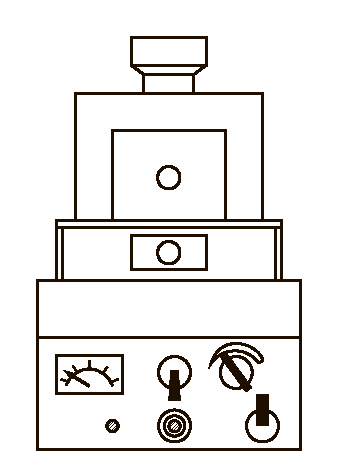
\includegraphics[width=.4\textwidth]{appearance} \hspace*{2em}
        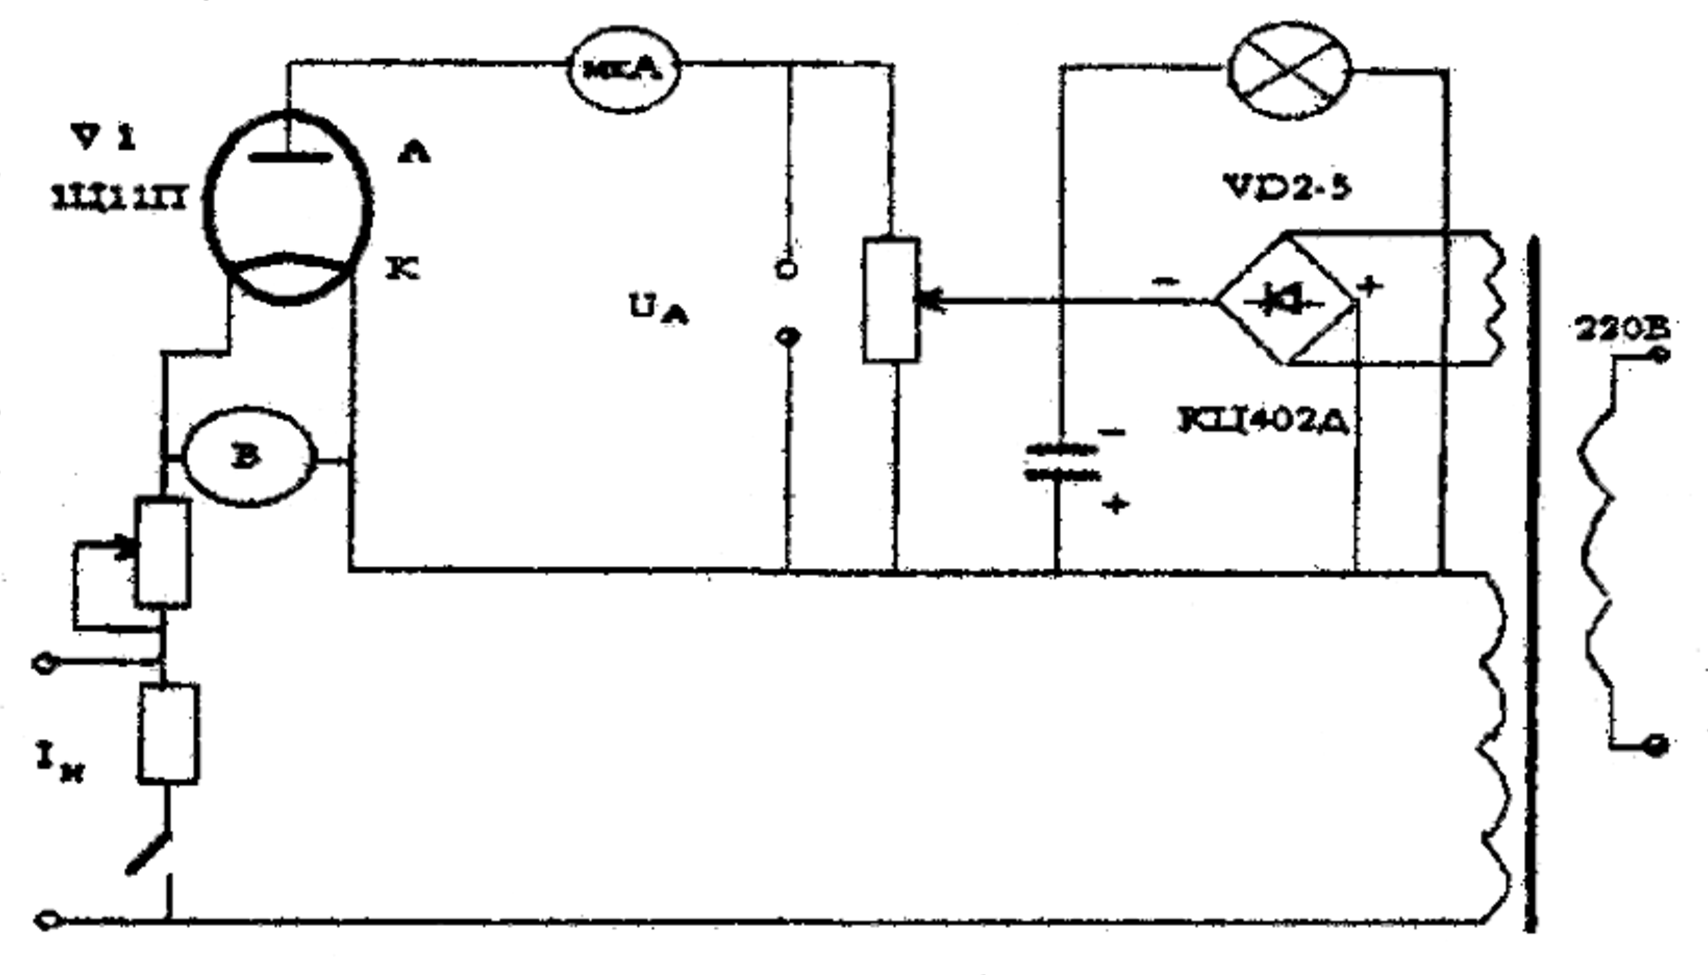
\includegraphics[width=.4\textwidth]{scheme} \\[.5em]
        \parbox{.4\textwidth}{\caption{Внешний вид установки}} \hspace*{2em}
        \parbox{.4\textwidth}{\caption{Принципиальная схема}}
    \end{figure}
    \vspace*{-2em}
    
    \begin{table}[h!]
        \center \caption{Результаты измерений и вычислений постоянной
        Стефана-Больцмана в первом опыте}
        \begin{tabular}{|*{9}{C{.08}|}} \hline
            \multicolumn{5}{|c|}{Температура} &
                \multirow{3}{*}{Ток \( J \)} &
                \multirow{2}{*}{Напря-} &
                \multirow{3}{*}{\( \sigma \)} &
                \multirow{3}{*}{\( \midnum{\sigma} \)} \\ \cline{1-5}
            яркостная \( t_s \) & истинная \( t \) &
                истинная \( T \) & воздуха \( t_0 \) &
                воздуха \( T_0 \) &&
                жение \( U \) && \\ \hline
            \( \vphantom{C}^{\circ}\!C \) &
                \( \vphantom{C}^{\circ}\!C \) &
                \( K \) & \( \vphantom{C}^{\circ}\!C \) &
                \( K \) & \( A \) & \( B \) &
                \( \cfrac{\text{Вт}}{\text{м}^2K^4} \) &
                \( \cfrac{\text{Вт}}{\text{м}^2K^4} \) \\[.5em] \hline
            1200 & 1283 &&&&&&& \\
            1300 & 1394 &&&&&&& \\
            1400 & 1508 &&&&&&& \\
            1500 & 1621 &&&&&&& \\
            1600 & 1736 &&&&&&& \\
            1700 & 1851 &&&&&&& \\ \hline
        \end{tabular}
    \end{table}
    
    \begin{table}[h!]
        \center \caption{Результаты измерений и вычислений постоянной
        Стефана-Больцмана во втором опыте}
        \begin{tabular}{|*{9}{C{.08}|}} \hline
            \multicolumn{5}{|c|}{Температура} &
                \multirow{3}{*}{Ток \( J \)} &
                \multirow{2}{*}{Напря-} &
                \multirow{3}{*}{\( \sigma \)} &
                \multirow{3}{*}{\( \midnum{\sigma} \)} \\ \cline{1-5}
            яркостная \( t_s \) & истинная \( t \) &
                истинная \( T \) & воздуха \( t_0 \) &
                воздуха \( T_0 \) &&
                жение \( U \) && \\ \hline
            \( \vphantom{C}^{\circ}\!C \) &
                \( \vphantom{C}^{\circ}\!C \) &
                \( K \) & \( \vphantom{C}^{\circ}\!C \) &
                \( K \) & \( A \) & \( B \) &
                \( \cfrac{\text{Вт}}{\text{м}^2K^4} \) &
                \( \cfrac{\text{Вт}}{\text{м}^2K^4} \) \\[.5em] \hline
            1200 & 1283 &&&&&&& \\
            1300 & 1394 &&&&&&& \\
            1400 & 1508 &&&&&&& \\
            1500 & 1621 &&&&&&& \\
            1600 & 1736 &&&&&&& \\
            1700 & 1851 &&&&&&& \\ \hline
        \end{tabular}
    \end{table}
    
    \pagebreak
    
    \begin{table}[h!]
        \center \caption{Результаты измерений и вычислений постоянной
        Стефана-Больцмана в третьем опыте}
        \begin{tabular}{|*{9}{C{.08}|}} \hline
            \multicolumn{5}{|c|}{Температура} &
                \multirow{3}{*}{Ток \( J \)} &
                \multirow{2}{*}{Напря-} &
                \multirow{3}{*}{\( \sigma \)} &
                \multirow{3}{*}{\( \midnum{\sigma} \)} \\ \cline{1-5}
            яркостная \( t_s \) & истинная \( t \) &
                истинная \( T \) & воздуха \( t_0 \) &
                воздуха \( T_0 \) &&
                жение \( U \) && \\ \hline
            \( \vphantom{C}^{\circ}\!C \) &
                \( \vphantom{C}^{\circ}\!C \) &
                \( K \) & \( \vphantom{C}^{\circ}\!C \) &
                \( K \) & \( A \) & \( B \) &
                \( \cfrac{\text{Вт}}{\text{м}^2K^4} \) &
                \( \cfrac{\text{Вт}}{\text{м}^2K^4} \) \\[.5em] \hline
            1200 & 1283 &&&&&&& \\
            1300 & 1394 &&&&&&& \\
            1400 & 1508 &&&&&&& \\
            1500 & 1621 &&&&&&& \\
            1600 & 1736 &&&&&&& \\
            1700 & 1851 &&&&&&& \\ \hline
        \end{tabular}
    \end{table}
    
    \begin{table}[h!]
        \center \caption{Результаты измерений и вычислений постоянной
        Стефана-Больцмана в четвертом опыте}
        \begin{tabular}{|*{9}{C{.08}|}} \hline
            \multicolumn{5}{|c|}{Температура} &
                \multirow{3}{*}{Ток \( J \)} &
                \multirow{2}{*}{Напря-} &
                \multirow{3}{*}{\( \sigma \)} &
                \multirow{3}{*}{\( \midnum{\sigma} \)} \\ \cline{1-5}
            яркостная \( t_s \) & истинная \( t \) &
                истинная \( T \) & воздуха \( t_0 \) &
                воздуха \( T_0 \) &&
                жение \( U \) && \\ \hline
            \( \vphantom{C}^{\circ}\!C \) &
                \( \vphantom{C}^{\circ}\!C \) &
                \( K \) & \( \vphantom{C}^{\circ}\!C \) &
                \( K \) & \( A \) & \( B \) &
                \( \cfrac{\text{Вт}}{\text{м}^2K^4} \) &
                \( \cfrac{\text{Вт}}{\text{м}^2K^4} \) \\[.5em] \hline
            1200 & 1283 &&&&&&& \\
            1300 & 1394 &&&&&&& \\
            1400 & 1508 &&&&&&& \\
            1500 & 1621 &&&&&&& \\
            1600 & 1736 &&&&&&& \\
            1700 & 1851 &&&&&&& \\ \hline
        \end{tabular}
    \end{table}
    
    \subsection{Подсчет погрешности и окончательные результаты}
    \center
    \rule{.95\textwidth}{.5pt} \\ \rule{.95\textwidth}{.5pt}
    \rule{.95\textwidth}{.5pt} \\ \rule{.95\textwidth}{.5pt}
    \rule{.95\textwidth}{.5pt} \\ \rule{.95\textwidth}{.5pt}
    \rule{.95\textwidth}{.5pt} \\ \rule{.95\textwidth}{.5pt}
    \rule{.95\textwidth}{.5pt} \\ \rule{.95\textwidth}{.5pt} \\
    \vspace*{2em}
    
    \emph{Вывод:} \rule{.885\textwidth}{.5pt}
    \rule{.95\textwidth}{.5pt} \\ \rule{.95\textwidth}{.5pt}
    \rule{.95\textwidth}{.5pt}
\end{document}
